\documentclass[a4paper,12pt]{article}

\usepackage [utf8]{inputenc}
\usepackage[T1]{fontenc}
\usepackage{fullpage}

\usepackage{subcaption}
\usepackage{tikz,tkz-graph}

\begin{document}


\begin{figure}[h]
  \centering
  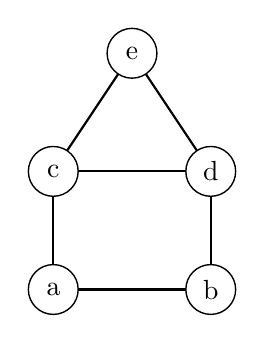
\begin{tikzpicture}
    % Vertices
      \Vertex[x=0 ,y=0]{a}
      \Vertex[x=2 ,y=0]{b}
      \Vertex[x=0 ,y=1.5]{c}
      \Vertex[x=2 ,y=1.5]{d}
      \Vertex[x=1 ,y=3]{e}

      % Edges
      \Edge(a)(b)
      \Edge(a)(c)
      \Edge(b)(d)    
      \Edge(c)(d)
      \Edge(c)(e)
      \Edge(d)(e)
  \end{tikzpicture}
  \caption{Graphe dont on doit trouver les arbres couvrants}
  \label{fig:grapheACouvrir}
\end{figure}


\begin{figure}[h]
  \centering
  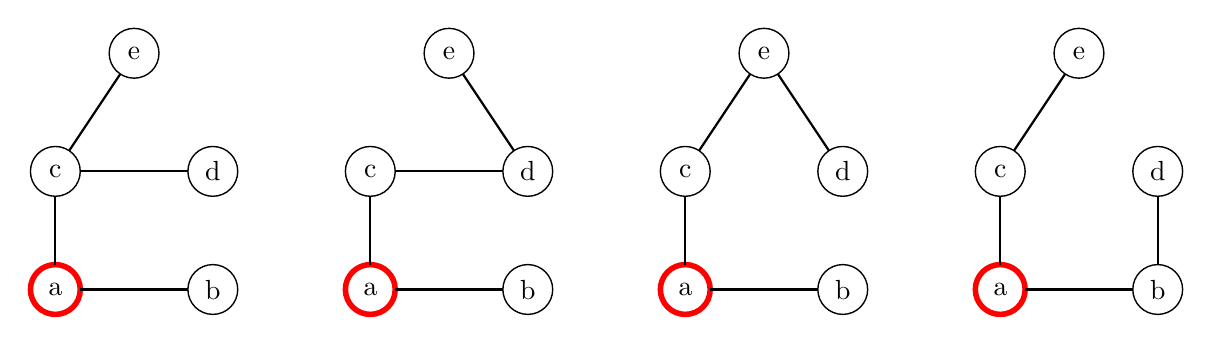
\begin{tikzpicture}%[scale=0.8]
    % Arbo 1 a-b + a-c
    
    % Arbo 1.1
    % Vertices
    \SetVertexNormal[LineWidth = 2pt, LineColor = red]
    \Vertex[x=0 ,y=0]{a}
    \SetVertexNormal
    \Vertex[x=2 ,y=0]{b}
    \Vertex[x=0 ,y=1.5]{c}
    \Vertex[x=2 ,y=1.5]{d}
    \Vertex[x=1 ,y=3]{e}

    % Edges
    \Edge(a)(b)
    \Edge(a)(c)
    \Edge(c)(d)
    \Edge(c)(e)
    
    % Arbo 1.2
    % Vertices
    \SetVertexNormal[LineWidth = 2pt, LineColor = red]
    \Vertex[x=4 ,y=0]{a}
    \SetVertexNormal
    \Vertex[x=6 ,y=0]{b}
    \Vertex[x=4 ,y=1.5]{c}
    \Vertex[x=6 ,y=1.5]{d}
    \Vertex[x=5 ,y=3]{e}

    % Edges
    \Edge(a)(b)
    \Edge(a)(c)
    \Edge(c)(d)
    \Edge(d)(e)

    % Arbo 1.3
    % Vertices
    \SetVertexNormal[LineWidth = 2pt, LineColor = red]
    \Vertex[x=8 ,y=0]{a}
    \SetVertexNormal
    \Vertex[x=10 ,y=0]{b}
    \Vertex[x=8 ,y=1.5]{c}
    \Vertex[x=10 ,y=1.5]{d}
    \Vertex[x=9 ,y=3]{e}

    % Edges
    \Edge(a)(b)
    \Edge(a)(c)
    \Edge(c)(e)
    \Edge(d)(e)

    % Arbo 1.4
    % Vertices
    \SetVertexNormal[LineWidth = 2pt, LineColor = red]
    \Vertex[x=12 ,y=0]{a}
    \SetVertexNormal
    \Vertex[x=14 ,y=0]{b}
    \Vertex[x=12 ,y=1.5]{c}
    \Vertex[x=14 ,y=1.5]{d}
    \Vertex[x=13 ,y=3]{e}

    % Edges
    \Edge(a)(b)
    \Edge(a)(c)
    \Edge(d)(b)
    \Edge(c)(e)

 \end{tikzpicture}
  \centering
  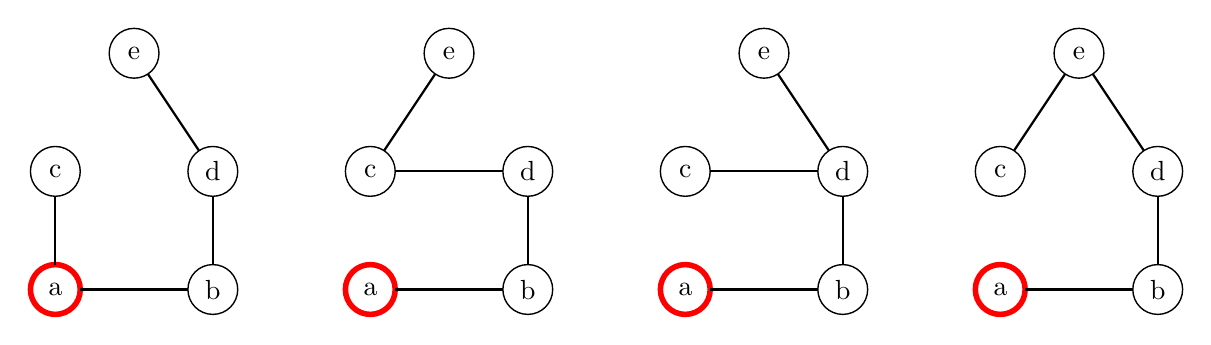
\begin{tikzpicture}
    % Arbo 1.5
    % Vertices
    \SetVertexNormal[LineWidth = 2pt, LineColor = red]
    \Vertex[x=0 ,y=0]{a}
    \SetVertexNormal
    \Vertex[x=2 ,y=0]{b}
    \Vertex[x=0 ,y=1.5]{c}
    \Vertex[x=2 ,y=1.5]{d}
    \Vertex[x=1 ,y=3]{e}

    % Edges
    \Edge(a)(b)
    \Edge(a)(c)
    \Edge(d)(b)
    \Edge(d)(e)

     % Arbo 2 a-b - a-c
    
    % Arbo 2.1
    % Vertices
    \SetVertexNormal[LineWidth = 2pt, LineColor = red]
    \Vertex[x=4 ,y=0]{a}
    \SetVertexNormal
    \Vertex[x=6 ,y=0]{b}
    \Vertex[x=4 ,y=1.5]{c}
    \Vertex[x=6 ,y=1.5]{d}
    \Vertex[x=5 ,y=3]{e}

    % Edges
    \Edge(a)(b)
    \Edge(b)(d)
    \Edge(c)(d)
    \Edge(c)(e)
    
    % Arbo 2.2
    % Vertices
   \SetVertexNormal[LineWidth = 2pt, LineColor = red]
    \Vertex[x=8 ,y=0]{a}
    \SetVertexNormal
    \Vertex[x=10 ,y=0]{b}
    \Vertex[x=8 ,y=1.5]{c}
    \Vertex[x=10 ,y=1.5]{d}
    \Vertex[x=9 ,y=3]{e}


    % Edges
    \Edge(a)(b)
    \Edge(b)(d)
    \Edge(c)(d)
    \Edge(d)(e)

    % Arbo 2.3
    % Vertices
     \SetVertexNormal[LineWidth = 2pt, LineColor = red]
    \Vertex[x=12 ,y=0]{a}
    \SetVertexNormal
    \Vertex[x=14 ,y=0]{b}
    \Vertex[x=12 ,y=1.5]{c}
    \Vertex[x=14 ,y=1.5]{d}
    \Vertex[x=13 ,y=3]{e}
    
    % Edges
    \Edge(a)(b)
    \Edge(b)(d)
    \Edge(c)(e)
    \Edge(d)(e)

  \end{tikzpicture}
  \centering
  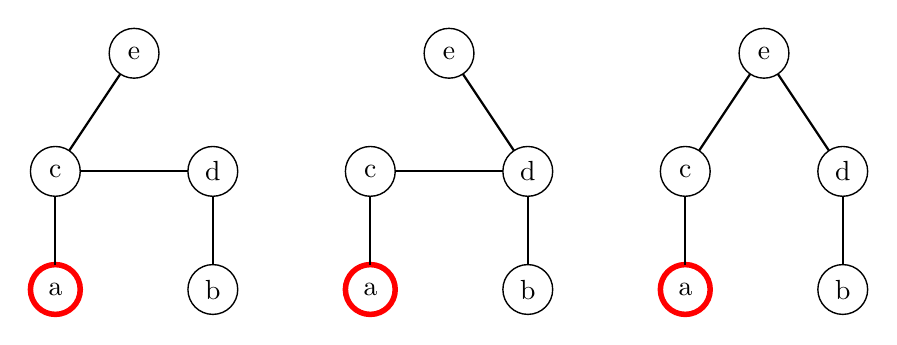
\begin{tikzpicture} 
    % Arbo 3  - a-b + a-c
    % Arbo 3.1
    % Vertices
    \SetVertexNormal[LineWidth = 2pt, LineColor = red]
    \Vertex[x=0 ,y=0]{a}
    \SetVertexNormal
    \Vertex[x=2 ,y=0]{b}
    \Vertex[x=0 ,y=1.5]{c}
    \Vertex[x=2 ,y=1.5]{d}
    \Vertex[x=1 ,y=3]{e}
    
    % Edges
    \Edge(a)(c)
    \Edge(b)(d)
    \Edge(c)(d)
    \Edge(c)(e)
    
    % Arbo 3.2
    % Vertices
    \SetVertexNormal[LineWidth = 2pt, LineColor = red]
    \Vertex[x=4 ,y=0]{a}
    \SetVertexNormal
    \Vertex[x=6 ,y=0]{b}
    \Vertex[x=4 ,y=1.5]{c}
    \Vertex[x=6 ,y=1.5]{d}
    \Vertex[x=5 ,y=3]{e}

    % Edges
    \Edge(a)(c)
    \Edge(d)(b)
    \Edge(c)(d)
    \Edge(d)(e)

    % Arbo 3.3
    % Vertices
    \SetVertexNormal[LineWidth = 2pt, LineColor = red]
    \Vertex[x=8 ,y=0]{a}
    \SetVertexNormal
    \Vertex[x=10 ,y=0]{b}
    \Vertex[x=8 ,y=1.5]{c}
    \Vertex[x=10 ,y=1.5]{d}
    \Vertex[x=9 ,y=3]{e}

    % Edges
    \Edge(a)(c)
    \Edge(c)(e)
    \Edge(d)(e)
    \Edge(d)(b)
  \end{tikzpicture}
  \caption{Arborescences de racine $a$ pour le graphe de la figure~\ref{fig:grapheACouvrir}}
  \label{fig:arboGraphe}
\end{figure}


\begin{figure}[h!]
  \begin{subfigure}[a]{\textwidth}
    \centering
    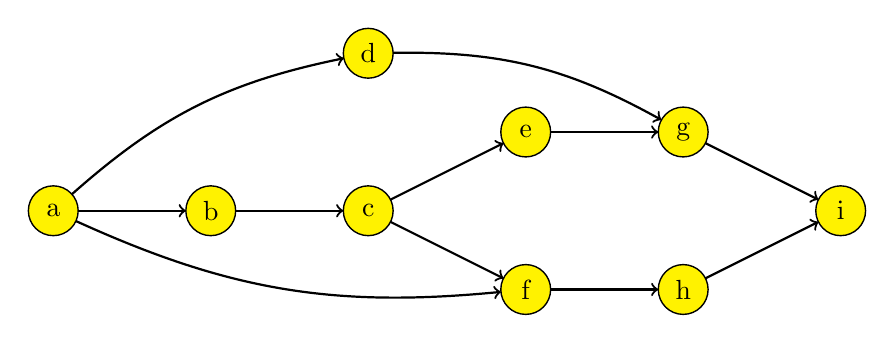
\begin{tikzpicture}
      % Vertices
      \SetVertexNormal[FillColor = yellow]
      \Vertex[x=0 ,y=1]{a}
      \Vertex[x=2 ,y=1]{b}
      \Vertex[x=4 ,y=1]{c}
      \Vertex[x=4 ,y=3]{d}
      \Vertex[x=6 ,y=2]{e}
      \Vertex[x=6 ,y=0]{f}
      \Vertex[x=8 ,y=2]{g}
      \Vertex[x=8 ,y=0]{h}
      \Vertex[x=10 ,y=1]{i}

      % Edges
      \tikzset{EdgeStyle/.style = {->}}
      \Edge(a)(b)
      \Edge(b)(c)
      \Edge(c)(e)    
      \Edge(c)(f)
      \Edge(e)(g)
      \Edge(f)(h)
      \Edge(g)(i)
      \Edge(h)(i)
      \tikzset{EdgeStyle/.style = {->,bend right=15}}
      \Edge[style={->}](a)(f)
      \tikzset{EdgeStyle/.style = {->,bend left=15}}
      \Edge[style={->}](a)(d)
      \Edge[style={->}](d)(g)        
    \end{tikzpicture}
    \caption{Graphe orienté sans circuit}
  \end{subfigure}

  \begin{subfigure}[b]{\textwidth}
    \centering
    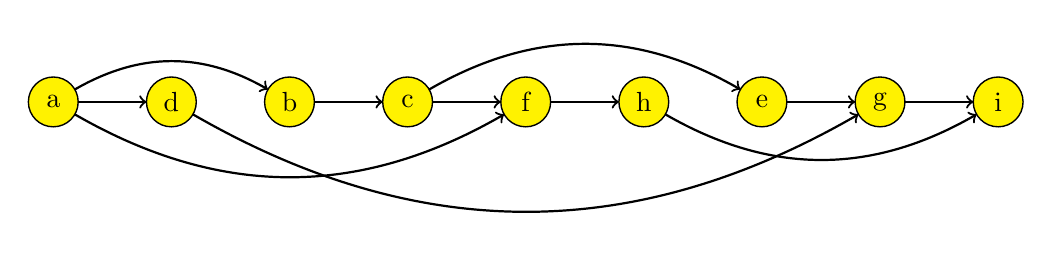
\begin{tikzpicture}
            % Vertices
      \SetVertexNormal[FillColor = yellow]
      \Vertex[x=0 ,y=1]{a}
      \Vertex[x=1.5 ,y=1]{d}
      \Vertex[x=3 ,y=1]{b}
      \Vertex[x=4.5 ,y=1]{c}
      \Vertex[x=6 ,y=1]{f}
      \Vertex[x=7.5 ,y=1]{h}
      \Vertex[x=9 ,y=1]{e}
      \Vertex[x=10.5 ,y=1]{g}
      \Vertex[x=12 ,y=1]{i}

      % Edges
      \tikzset{EdgeStyle/.style = {->}}
      \Edge(a)(d)
      \Edge(b)(c)
      \Edge(c)(f)
      \Edge(e)(g)
      \Edge(f)(h)
      \Edge(g)(i)
      \tikzset{EdgeStyle/.style = {->,bend right=30}}
      \Edge(a)(f)
      \Edge(h)(i)
      \Edge(d)(g)
      \tikzset{EdgeStyle/.style = {->,bend left=30}}
      \Edge(c)(e)    
      \Edge(a)(b)
    \end{tikzpicture}
    \caption{Représentation compatible avec un tri topologique}
  \end{subfigure}
  \caption{Exemple de graphe sans circuit avec un tri topologique}
  \label{fig:ExempleTopo}
\end{figure}


\begin{figure}[h!]
  \centering
  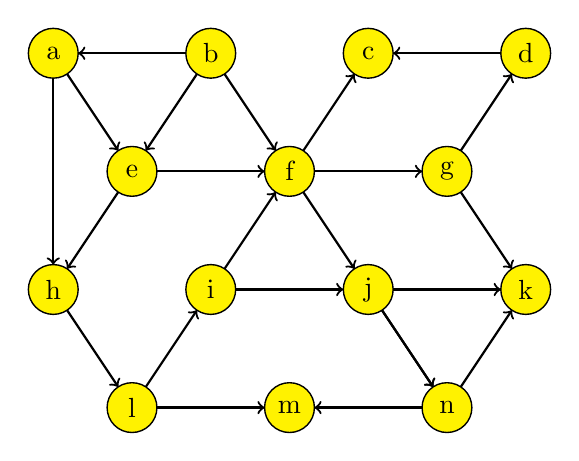
\begin{tikzpicture}
      % Vertices
      \SetVertexNormal[FillColor = yellow]
      \Vertex[x=0 ,y=4.5]{a}
      \Vertex[x=2 ,y=4.5]{b}
      \Vertex[x=4 ,y=4.5]{c}
      \Vertex[x=6 ,y=4.5]{d}
      \Vertex[x=1 ,y=3]{e}
      \Vertex[x=3 ,y=3]{f}
      \Vertex[x=5 ,y=3]{g}
      \Vertex[x=0 ,y=1.5]{h}
      \Vertex[x=2 ,y=1.5]{i}
      \Vertex[x=4 ,y=1.5]{j}
      \Vertex[x=6 ,y=1.5]{k}
      \Vertex[x=1 ,y=0]{l}
      \Vertex[x=3 ,y=0]{m}
      \Vertex[x=5 ,y=0]{n}
      
      % Edges
      \tikzset{EdgeStyle/.style = {->}}
      \Edge(b)(a)
      \Edge(a)(e)
      \Edge(a)(h)    
      \Edge(b)(e)
      \Edge(b)(f)
      \Edge(d)(c)
      \Edge(e)(f)
      \Edge(e)(h)
      \Edge(f)(g)
      \Edge(f)(j)
      \Edge(f)(c)
      \Edge(g)(k)
      \Edge(g)(d)
      \Edge(i)(f)
      \Edge(i)(j)
      \Edge(j)(n)
      \Edge(j)(k)
      \Edge(h)(l)
      \Edge(l)(i)
      \Edge(j)(n)
      \Edge(l)(m)
      \Edge(n)(m)
      \Edge(n)(k)
    \end{tikzpicture}
  \caption{Graphe à trier topologiquement} 
  \label{fig:grapheTopo}
\end{figure}




\end{document}

